\documentclass[a4paper,twocolumn]{article}

\usepackage{color}
\usepackage{appendix}

\usepackage{amsmath}

\usepackage{listings}
\usepackage{graphicx}
\usepackage[sc]{mathpazo} % Use the Palatino font
\usepackage[T1]{fontenc} % Use 8-bit encoding that has 256 glyphs
\usepackage[utf8]{inputenc} % Use utf-8 as encoding
\linespread{1.05} % Line spacing - Palatino needs more space between lines
\usepackage{microtype} % Slightly tweak font spacing for aesthetics

\usepackage[spanish]{babel} % Language hyphenation and typographical rules
%\usepackage[galician]{babel} % Change to this if using galician

\usepackage[hmarginratio=1:1,top=32mm,columnsep=20pt]{geometry} % Document margins
\usepackage[hang, small,labelfont=bf,up,textfont=it,up]{caption} % Custom captions under/above floats in tables or figures
\usepackage{booktabs} % Horizontal rules in tables

\usepackage{enumitem} % Customized lists
\setlist[itemize]{noitemsep} % Make itemize lists more compact

\usepackage{parskip}

\usepackage{abstract} % Allows abstract customization
\renewcommand{\abstractnamefont}{\normalfont\bfseries} % Set the "Abstract" text to bold
\renewcommand{\abstracttextfont}{\normalfont\small\itshape} % Set the abstract itself to small italic text

\usepackage{titlesec} % Allows customization of titles
\renewcommand\thesection{\Roman{section}} % Roman numerals for the sections
\renewcommand\thesubsection{\Alph{subsection}} % roman numerals for subsections
\titleformat{\section}[block]{\large\scshape\centering}{\thesection.}{1em}{} % Change the look of the section titles
\titleformat{\subsection}[block]{\large}{\thesubsection.}{1em}{} % Change the look of the section titles

\usepackage{fancyhdr} % Headers and footers
\pagestyle{fancy} % All pages have headers and footers
\fancyhead{} % Blank out the default header
\fancyfoot{} % Blank out the default footer
%\fancyhead[C]{Running title $\bullet$ May 2016 $\bullet$ Vol. XXI, No. 1} % Custom header text
\fancyfoot[C]{\thepage} % Custom footer text

\usepackage{titling} % Customizing the title section

\usepackage{hyperref} % For hyperlinks in the PDF

\usepackage[verbose]{placeins}

\usepackage{adjustbox}

%----------------------------------------------------------------------------------------
%	TITLE SECTION
%----------------------------------------------------------------------------------------

\setlength{\droptitle}{-5\baselineskip} % Move the title up

%\pretitle{\begin{center}\huge\bfseries} % Article title formatting
%\posttitle{ \end{center} } % Article title closing formatting

\title{
    \begin{center}
        \huge\bfseries Procesadores del lenguaje, bloque 2: Un acercamiento a la IA
    \end{center}
} % Article title

\preauthor{\setlength{\parskip}{20pt}}

\postauthor{\setlength{\parskip}{1pt}}


\author{%
    \begin{center}
        \large\centering\textsc{Marcelo Fort Muñoz} \\[1ex] % Your name
        \normalsize Procesadores del lenguaje \\[0.25ex]
        \normalsize Universidad de Nebrija (Grupo A2) \\[0.25ex] % Your institution
        \normalsize \{mfortm\}@alumnos.nebrija.es % Your email address
        %\and % Uncomment if 2 authors are required, duplicate these 4 lines if more
        %\textsc{Jane Smith}\thanks{Corresponding author} \\[1ex] % Second author's name
        %\normalsize University of Utah \\ % Second author's institution
        %\normalsize \href{mailto:jane@smith.com}{jane@smith.com} % Second author's email address
    \end{center}
}

\predate{\setlength{\parskip}{5pt}}
\postdate{\setlength{\parskip}{1pt}}

\date{\begin{center}
          \large\today\\[2.5ex]
\end{center}} % Leave empty to omit a date

\renewcommand{\maketitlehookd}{%
    \begin{abstract}
        \setlength{\parskip}{22pt}
        \noindent En la inteligencia artificial se procesan textos para crear modelos estadísticos que puedan analizarlos,
        predecirlos o ejecutar todo tipo de acciones sobre ellos. Para hacer esto, es necesario procesar previamente el texto,
        aplicándole distintas técnicas de normalización, tokenización, análisis sintáctico, etc.
        \\\mbox{}\\
        \textbf{\textit{Palabras clave}: Aquí las palabras clave}
        \setlength{\parskip}{10pt}
    \end{abstract}

}

%----------------------------------------------------------------------------------------

\definecolor{dkgreen}{rgb}{0,0.6,0}
\definecolor{gray}{rgb}{0.5,0.5,0.5}
\definecolor{mauve}{rgb}{0.58,0,0.82}

%\lstset{frame=tb,
%    language=C,
%    aboveskip=3mm,
%    belowskip=3mm,
%    showstringspaces=false,
%    columns=flexible,
%    basicstyle={\small\ttfamily},
%    numbers=none,
%    numberstyle=\tiny\color{gray},
%    keywordstyle=\color{blue},
%    commentstyle=\color{dkgreen},
%    stringstyle=\color{mauve},
%    breaklines=true,
%    breakatwhitespace=true,
%    tabsize=3
%}



\begin{document}

    % Print the title
    \maketitle

    \parskip=0.5\baselineskip \advance\parskip by 0pt plus 1pt
%\setlength{\parskip}{1pt}
%----------------------------------------------------------------------------------------
    %	ARTICLE CONTENTS
    %----------------------------------------------------------------------------------------


    \section{Introducción}\label{sec:introduccion}


    \section{Metodología y funcionamiento}\label{sec:metodologia-y-funcionamiento}
    Normalizar el texto es un paso previo a cualquier procesamiento de lenguaje natural.
    En nuestro caso, por simplicidad, hemos considerado que la normalización se compone de ocho pasos \cite{enunciado}:

    \begin{enumerate}

        \item {Lowercasing} Convertir todo el texto a minúsculas.
        Esta operación reduce dimensiones al convertir en la misma palabra aquellas cadenas que sólo se diferencian por mayúsculas.

        \item {Eliminar puntuación} Eliminar signos de puntuación innecesarios.
        Esta operación dependerá del contexto específico, pero en general, al eliminar la puntuación, se reduce el ruido en el texto quitando
        símbolos no muy importantes para el significado del texto.

        \item {Eliminar números} Remover los números que no aporten valor al análisis.
        Una variante de esta operación sería convertir los números a palabras, pero en nuestro caso, hemos optado por eliminar.

        \item {Eliminar stop words} Filtrar palabras comunes que no aportan información.
        Otra vez, esta operación dependerá del contexto, pero en general, se eliminan palabras comunes que no aportan información relevante al análisis.

        \item {Lematización} Reducir las palabras a su forma base.
        Esta operación reduce la dimensionalidad del texto, ya que reduce las palabras a su forma base.
        Es más «fina» que la operación de stemming, pero requiere más recursos computacionales y suele tener dependencias de librerías externas o componentes como POS («Part of Speech»)\cite{ibm_pos}

        \item {Stemming} Aplicar stemming si la librería lo soporta.
        Es el «primo bruto» de la lematización, ya que reduce las palabras a su raíz.
        Esto lo hace eliminando sufijos y prefijos mediante reglas predefinidas\cite{ibm_pos}.

        \item {Corrección ortográfica} Corregir errores ortográficos en el texto.

        \item {Tokenización} Dividir el texto en tokens.

    \end{enumerate}

    \newpage

    \subsection{Librerias}\label{subsec:libs}
    Para la implementación de los pasos de normalización, se ha utilizado el lenguaje de programación Python y diferentes librerías.
    Las librerías usadas son NLTK, Spacy, TextBlob y GenSim\footnote{Gensim no es una librería, sino un framework}.

    \begin{table}[h]
        \centering

        \begin{adjustbox}{max width=\textwidth/2}

            \begin{tabular}{lllllllll}
                \toprule
                \textbf{Nombre} & \textbf{Lowercasing} & \textbf{Puntuación} & \textbf{Números} & \textbf{Stop-Words} & \textbf{Lemma} & \textbf{Stemm} & \textbf{Corrección} & \textbf{Tokenización} \\
                \midrule
                Gensim          & Sí                   & Sí                  & Sí               & Sí                  & Dep.           & Sí             & No                  & Sí                    \\
                SpaCy           & No                   & Sí                  & Sí               & Sí                  & Sí             & No             & Dep.                & Sí                    \\
                TextBlob        & Sí                   & Sí                  & No               & Dep.                & Sí             & Sí             & Sí                  & Sí                    \\
                NLTK            & No                   & No                  & No               & Sí                  & Sí             & Sí             & No                  & Sí                    \\
                \bottomrule
            \end{tabular}
        \end{adjustbox}
        \caption{funcionalidades implementadas en cada librería}
        \label{tab:libsCapac}
    \end{table}


    En la \autoref{tab:libsCapac} se puede ver un resumen de las funcionalidades implementadas en cada librería.
    Dep. significa que la funcionalidad depende de la librería o de un componente externo.
    Para que la comparación fuese más justa y sencilla, todas las librerías hacen todas las operaciones y usan los mismos datos de entrada.
    Se han usado los textos del libro de Dovstoyevski «El idiota»\cite{Dovstoyevski.theidiot} para hacer las pruebas y se ha intentado usar los mismos componentes externos para llenar los huecos en las funcionalidades.

    \subsection {Diferencias entre librerías}\label{subsec:diflibs}
    Las diferencias entre las librerías son notables.
    Sobre todo entre NLTK y TextBlob frente a Gensim y SpaCy.
    En los siguientes apartados se detallarán las diferencias entre las librerías.

    \subsubsection{Documentación}\label{subsubsec:doc}
    A la hora de buscar documentación, NLTK es la clara ganadora.
    No sólo porque es la más antigua, sino porque tiene publicado un libro de aproximación y uso avanzado\cite{bird2009natural}.

    TextBlob (que usa NLTK como parte de su «columna vertebral»), también tiene una buena documentación\cite{textblobdocs}.
    Esta librería es muy fácil de usar y tiene una API muy sencilla.

    Spacy \cite{spacydocs} también tiene una documentación comprensiva, pero comete el fallo de asumir conocimientos técnicos que el usuario puede no tener.
    Aunque es una librería muy potente, su curva de aprendizaje es más pronunciada que la de NLTK o TextBlob.
    Es de justicia, de todos modos, decir que Spacy es una librería más enfocada a la industria y sector profesional.

    Gensim \cite{gensimdocs} tiene la documentación más difícil, debido a que, por un lado, está un poco escondida y, por otro lado, asume más conocimientos técnicos que las otras librerías.
    Aun así, está diseñada para funcionar «out of the box» y es muy potente.

    \subsubsection{Facilidad de uso}\label{subsubsec:facilidad}

    NLTK es la librería más fácil de usar.
    Tienen una API muy sencilla y es muy fácil de aprender.
    TextBlob es aún más sencilla, ya que es una capa de abstracción sobre NLTK.

    Spacy es más complicada de usar, porque se requiere de ciertos conocimientos técnicos de sistemas operativos (pipelines) que el usuario puede no tener.

    Gensim es la más complicada de usar, porque está diseñada para ser usada en entornos profesionales y de investigación.
    Aun así, es muy potente y tiene una API muy completa y permite ajustar mucho los algoritmos.

    \subsubsection{Diseño}\label{subsubsec:diseno}
    NLTK es la librería más antigua y se nota en su diseño.
    Es una librería muy completa y potente, utilizando una estructura de clases y funciones muy clásica.

    TextBlob es una capa de abstracción sobre NLTK, por lo que su diseño es muy similar.
    Este intenta simplificar el uso de NLTK y añadir funcionalidades que no tiene NLTK.
    Un ejemplo de esto es la corrección ortográfica, «lowercasing» y eliminación de puntuación, que no están en NLTK.

    Spacy, por otro lado, es directamente parte de otro paradigma.
    Está diseñada con el concepto de pipelines modulares, que permiten al usuario ajustar el procesamiento del texto a sus necesidades.
    Esto la hace más complicada de usar, pero más potente y flexible.
    Además en las últimas versiones se ha apuntado a la paralelización multiproceso.

    Gensim es una librería de procesamiento de texto muy potente.
    Está diseñada para el procesamiento de texto automático y «deep learning».

    \subsection{Fortalezas y debilidades de las librerías}\label{subsec:fortalezas-y-debilidades-de-las-librerias}

    \subsubsection{NLTK}\label{subsubsec:nltk}

    \textbf{Fortalezas:}
    \begin{itemize}
        \item Amplio abanico de herramientas para el procesamiento de texto.
        \item Mucha documentación y ejemplos disponibles.
    \end{itemize}

    \textbf{Debilidades:}
    \begin{itemize}
        \item Mantenimiento más difícil del código.
        \item Su uso en producción puede ser complicado.
    \end{itemize}

    \subsubsection{Spacy}\label{subsubsec:spacy}

    \textbf{Fortalezas:}
    \begin{itemize}
        \item Muy potente y flexible para grandes volúmenes de texto\footnote{https://spacy.io/usage/facts-figures}.
        \item Diseñada para el uso en producción.
        \item Implementada en \textit{C} (\textit{Cython})\cite{spacy.cython}
    \end{itemize}

    \textbf{Debilidades:}
    \begin{itemize}
        \item Curva de aprendizaje pronunciada.
        \item Requiere conocimientos técnicos.
        \item Menos documentación que NLTK y documentación obsoleta sin marcar disponible.
    \end {itemize}

    \subsubsection{TextBlob}\label{subsubsec:textblob}

    \textbf{Fortalezas:}
    \begin{itemize}
        \item Muy fácil de usar.
        \item API muy sencilla.
        \item Capa de abstracción sobre NLTK.
    \end {itemize}

    \textbf{Debilidades:}
    \begin{itemize}
        \item Depende de NLTK.
        \item Más lenta que NLTK.
    \end {itemize}

    \subsubsection{Gensim}\label{subsubsec:gensim}

    \textbf{Fortalezas:}
    \begin{itemize}
        \item Muy potente.
        \item Diseñada para el procesamiento de texto automático y \textit{deep learning}, por lo que se integra muy bien con otros frameworks.
        \item Optimizada para grandes volúmenes de texto.
    \end {itemize}

    \textbf{Debilidades:}
    \begin{itemize}
        \item Curva de aprendizaje pronunciada.
        \item Requiere conocimientos técnicos.
        \item Muy especializada, por lo que algunas funcionalidades pueden no estar disponibles.
    \end {itemize}

    \subsection{Implementación de la normalización}\label{subsec:implementacion-de-la-normalizacion}
    En esta sección se detallará las particularidades de la implementación \cite{marcelo.implementaciones} de la normalización en cada librería.

    \subsubsection{NLTK}\label{subsubsec:nltk_impl}
    En el caso de NLTK, se ha tenido que usar la clase \textit{Speller} de la librería \textit{autocorrect} para la corrección ortográfica.
    Esto se debe a que NLTK no tiene una funcionalidad de revisión ortográfica.

    La implementación con NLTK ha dependido mucho de los Strings de python, pero ha sido muy sencilla y rápida de hacer.

    \subsubsection{Spacy}\label{subsubsec:spacy_impl}
    Spacy ha sido la librería más complicada de implementar.
    Para usar correctamente Spacy añadiendo el módulo de comprobación ortográfica \textit{contextualSpellCheck} se ha tenido que añadir al pipeline.
    Sin embargo, dado como funciona Spacy, se ha añadido:
    \begin{lstlisting}[language=Python,label={lst:codigoSpellSpacy},basicstyle=\scriptsize]
nlp.disable_pipes("tagger", "lemmatizer")

if(not nlp.has_pipe("contextual spellchecker")):
    contextualSpellCheck.add_to_pipe(nlp)

    .
    .
    .

doc_corregido = list(nlp.pipe([texto_minusculas]))
    \end{lstlisting}

    Se puede notar el uso de la función \textit{disable\_pipes} para desactivar las tuberías no esenciales y el uso de \textit{has\_pipe} para comprobar si la tubería ya está añadida.
    Se deshabilitan las «tuberías» no esenciales para permitir que SpaCy funcione lo más rápido posible,
    ya que como tiene por principio no alterar el texto original, se da la correción por separado.

    Por esto, más tarde se dehabilita al corrector y se procesa el texto corregido.

    \begin{lstlisting}[language=Python,label={lst:codigoSpellSpacy2},basicstyle=\scriptsize]
nlp.remove_pipe("contextual spellchecker")

  nlp.enable_pipe("lemmatizer")
  nlp.enable_pipe("tagger")

  doc = list(nlp.pipe([texto_corregido]))
    \end{lstlisting}

    Depués, con los métodos específicos de SpaCy para los tokens, se filtran espacios, puntuación y numéricos.
    Finalmente, se devuelve el texto normalizado.

    \subsubsection{TextBlob}\label{subsubsec:textblob_impl}
    En el caso de TextBlob, el acercamiento ha sido mucho más rápido.
    Para empezar, el filtrado se hace automáticamente mediante la llamada \textit{TextBlob(var)}.
    Después, se corrige la ortografía con un método del objeto devuelto por la llamada anterior (\textit{var.correct().op1()...opn()}).

    Procedemos a lematizar y stemmerizar el texto, llama a los métodos \textit{lemmatize()} y \textit{stem()} respectivamente.
    Finalmente, con el véctor de stopwords y las Strings de Python, se filtran los stopwords y se devuelve el texto normalizado.

    Hay que tener en cuenta que TextBlob es una capa de abstracción sobre NLTK.
    Esto causa que TextBlob dependa de NLTK para muchas de sus funcionalidades.

    \subsubsection{Gensim}\label{subsubsec:gensim_impl}
    Gensim es una librería muy potente, pero muy especializada.
    Nota: Se han usado las pattern.en para lematizar y autocorrect para corregir la ortografía.
    Hay que decir que Gensim dejó caer el soporte a lematización a causa de su bajo uso y que Pattern.en era la implementación usada en la librería.

    La implementación con GenSim ha sido (exceptuando todo lo que no está implementado),
    una solución que podría haber sido de una línea. Con la llamada a \textit{preprocess\_string}.

    La falta de soporte para la corrección ortográfica y la lematización pueden ser interpretadas como una señal de que Gensim no es la librería adecuada para normalización de texto.




    \clearpage


%        \label{fig:menorOigual}
%    \end{figure}


%    \clearpage
%    \begin{figure}
%        \centering
%        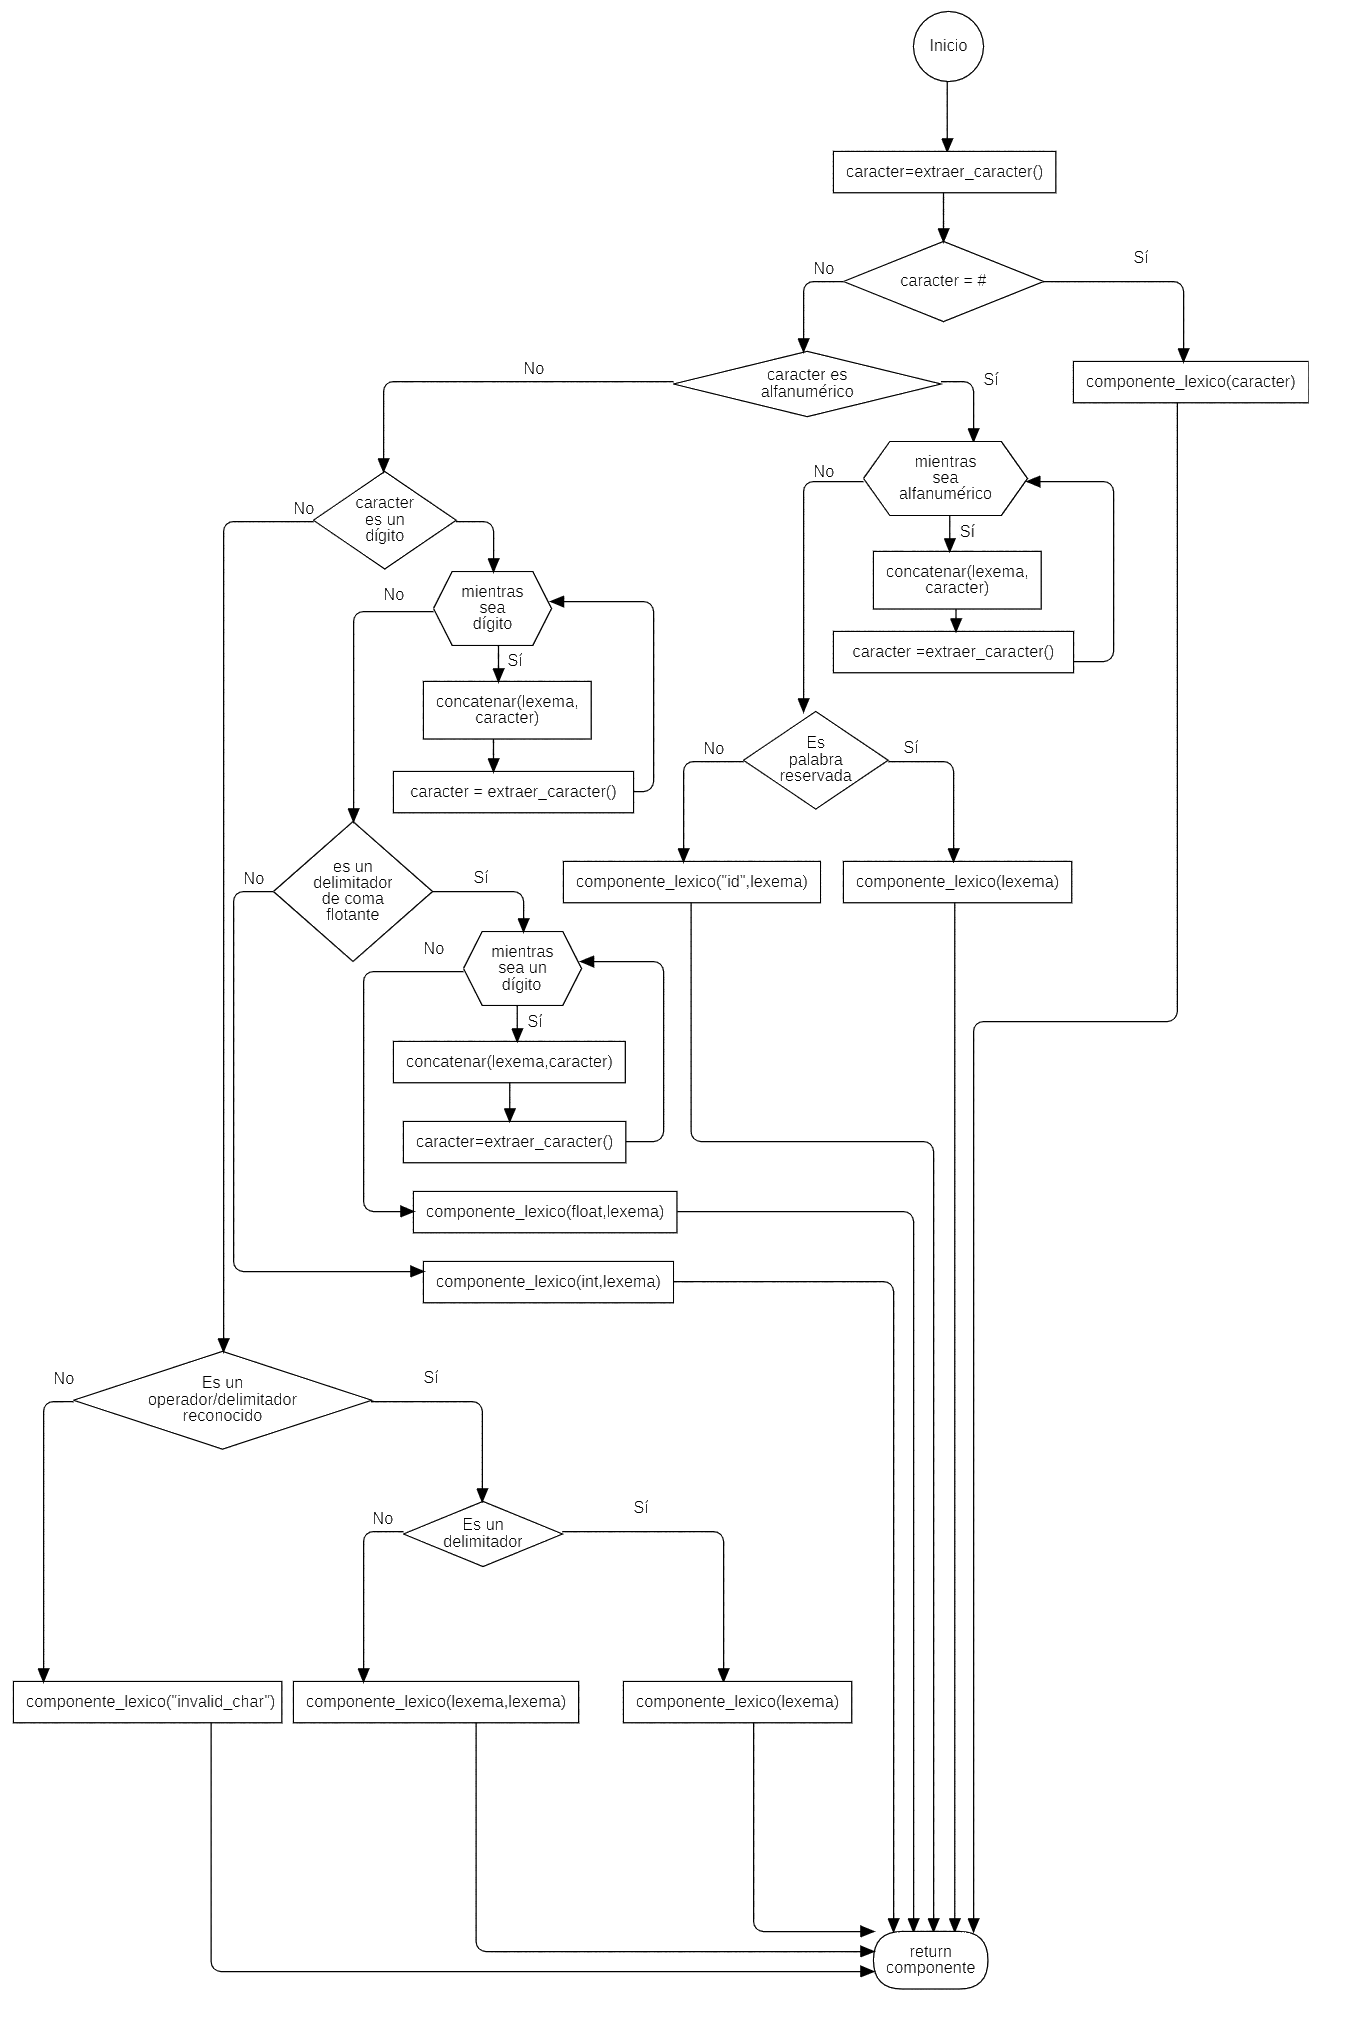
\includegraphics[width=1.00\linewidth]{diagramaFlujoDecisionCaracteresFinal}
%        \caption{Diagrama de flujo para la creación de un token}
%        \label{fig:diag 1}
%    \end{figure}


    \section{Modificaciones realizadas a la gramática original}\label{sec:modificaciones-realizadas-a-la-gramatica-original}

    \subsection {Eliminando la recursión a la izquierda}\label{subsec:eliminando-la-recursion-a-la-izquierda}
    En esta sección se detallará como se modificó la gramática para eliminar la recursividad a la izquierda.


    Como se puede ver en la \autoref{fig:gramatica_original}, existe recursividad a la izquierda en las producciones de expresión:
    \begin{align}
        &\text{expresión} \rightarrow \text{expresión} + \text{término} \\
        &\text{expresión} \rightarrow \text{expresión} - \text{término}
    \end{align}

    También existe esa recursividad hacia la izquierda en las producciones de término:

    \begin{align}
        &\text{término} \rightarrow \text{término} * \text{factor} \\
        &\text{término} \rightarrow \text{término} / \text{factor}
    \end{align}

    Para eliminar dicha recursividad, se utilizará la fórmula{librodragon}:
    \begin{gather*}
        A \rightarrow \beta R\\
        R \rightarrow \alpha R \; \vert \; \epsilon
    \end{gather*}

    \subsubsection{Caso de expresión}
    En el caso de expresión, siguiendo las producciones originales de la \autoref{fig:gramatica_original}, podemos concluir que nuestros $ \alpha_i $ serán:
    \begin{align*}
        &\alpha_1 = + \: \text{término}\\
        &\alpha_2 = - \: \text{término}
    \end{align*}
    y $ \beta $ será:
    \[\beta = \text{término}\]

    Usando la fórmula antes señalada, nos quedarán las producciones no recursivas de la \autoref{fig:expr_nr_b}.

    \begin{figure}[h]
        \begin{align}
            &\text{expresión} \rightarrow \text{término} \; \text{expresión}' \\
            &\text{expresión}' \rightarrow + \; \text{término} \; \text{expresión}' \\
            &\vert \; - \; \text{término} \; \text{expresión}' \\
            &\vert \; \epsilon
        \end{align}

        \caption{Producciones de expresión sin recurrencia a la izquierda}
        \label{fig:expr_nr_b}
    \end{figure}

    \subsubsection{Caso de término}
    De la misma forma que para las producciones de expresión, primero extraemos los $\alpha$:
    \begin{align}
        \alpha_1 = * \; \text{factor}\nonumber \\
        \alpha_2 = / \; \text{factor}\nonumber
    \end{align}
    Para el caso de $\beta$:
    \begin{align}
        \beta = \text{factor} \nonumber
    \end{align}

    Usando esas $\alpha$ y $\beta$, se procesa la producción original en:

    \begin{figure}[ht]

        \begin{align}
            &\text{término} \rightarrow \text{factor} \; \text{término}' \\
            &\vert \; \text{término}' \rightarrow * \; \text{factor} \; \text{término}' \\
            &\vert \; / \; \text{factor} \; \text{término}'\\
            &\vert \; \epsilon
        \end{align}
        \caption{Producciones de término sin recurrencia a la izquierda}
        \label{fig:Term_nr_b}
    \end{figure}

    Como factor no tiene recursividad, lo dejamos como está.

    \subsubsection{Renombrado de producciones}
    Como ahora tenemos dos nuevas producciones llamadas \textit{expresión'} y \textit{término'}, para mayor facilidad de tratamiento, les cambiaremos el nombre.

    En el caso de \textit{expresión'}, como va después de \textit{término}, lo llamaremos \textit{más\_términos}.
    Para el caso de \textit{término'}, lo renombraremos como \textit{más\_factores}.

    \subsubsection{Resultado tras la eliminación de la recursividad}
    Tras eliminar la recursividad, obtenemos la gramática de la \autoref{fig:Term_nr_totales}

    \clearpage

    \begin{figure}
        \begin{align}
            \label{eqc:gramaticaCorregida}
            &\text{expresión} \rightarrow \text{término} \; \text{más\_términos} \\
            &\text{más\_términos} \rightarrow  + \;\text{término} \; \text{más\_términos}
            \refstepcounter{equation}\nonumber  \\
            &\vert \; - \text{término} \; \text{más\_términos} \\
            &\vert \; \epsilon \\
            &\text{término} \rightarrow \text{factor} \; \text{más\_factores} \\
            &\text{más\_factores} \rightarrow  * \;\text{factor} \; \text{más\_factores} \\
            &\vert \; / \; \text{factor} \; \text{más\_factores} \\
            &\vert \; \epsilon \\
            &\text{factor} \; \rightarrow (\text{expresión})\\
            &\vert \; num\label{eq:numSinRecursividad}
        \end{align}
        \caption{Gramática sin recursividad a la izquierda}
        \label{fig:Term_nr_totales}
    \end{figure}


    \section{Acciones añadidas a la gramática}\label{sec:acciones-anadidas-a-la-gramatica}
    Una vez modificada la gramática para que no haya producciones con recurrencia a la izquierda (\autoref{fig:Term_nr_totales}), procedemos a añadir acciones semánticas que nos permitan hacer la traducción guiada por la sintaxis.


    En primer lugar, se introducirá: pila(n.val) después de $num$\eqref{eq:numSinRecursividad}.
    Esto nos permitirá añadir los números en este caso a la pila.

    En los casos de más\_factores y mas\_términos, se hará una operación de pila (''<símbolo>'') («push»\footnote{en.wikipedia.org/wiki/Stack\_(abstract\_data\_type)}) con el correspondiente símbolo de cada producción entre factor y mas\_factores en el primer caso y entre término y mas\_términos en el último.

    La introducción en «el medio» no es «fortuita», ya que de esta forma la operación podrá ser la última de la expresión o simplemente de la operación matemática, permitiendo al imprimir la pila o al usarla obtener la cadena inicial en formato de notación polaca inversa.

    Esto es, porque al apilar los operadores y números en la lista de esta forma, al sacarlos son extraídos con el formato correcto.
    Supongamos que en una pila $P$ vacía.
    Insertando $7+5$ siguiendo la gramática, la inserción sería 7 $\rightarrow$ 5 $\rightarrow$ $+$ (el $+$ queda pendiente en su paso), quedando la pila como $P=\{7,5,+\}$, que al imprimir o evaluar sería: $7\,5 +.$

    \subsection{Resultado tras la adición de las acciones semánticas a la gramática}\label{subsec:resultado-tras-la-adicion-de-las-acciones-semanticas-a-la-gramatica}

    \begin{figure}[h]
        \begin{align}
            &\text{expresión} \rightarrow \text{término} \; \text{más\_términos} \\
            &\text{más\_términos} \rightarrow   \\
            &\qquad+ \;\text{término} \; \{\text{pila('+')}\} \; \text{más\_términos} \nonumber  \\
            &\vert \; - \text{término} \; \{\text{pila('-')}\} \text{más\_términos} \\
            &\vert \; \epsilon \\
            \nonumber\\
            &\text{término} \rightarrow \text{factor} \; \text{más\_factores} \\
            &\text{más\_factores} \rightarrow \\
            &\qquad * \;\text{factor} \;\{\text{pila('*')}\}\; \text{más\_factores} \nonumber \\
            &\vert \; / \; \text{factor} \; \{\text{pila('/')}\} \; \text{más\_factores} \\
            &\vert \; \epsilon \\
            \nonumber\\
            &\text{factor} \; \rightarrow (\text{expresión})\\
            &\vert \; num  \{\text{pila(num.val)}\}
        \end{align}
        \caption{Gramática con las acciones semánticas}
        \label{fig:GramaticaConAcciones}
    \end{figure}


    \clearpage


    \section{Conclusiones}\label{sec:conclusiones}
    En esta práctica, hemos implementado un analizador léxico y un analizador sintáctico para traducir expresiones aritméticas de notación infija a notación postfija, eliminando la recursividad por la izquierda en la gramática original.

    Para la traducción a notación postfija, hemos utilizado acciones semánticas en lugar de reglas semánticas.
    Las acciones semánticas resultaron ideales para esta tarea, ya que permiten una manipulación directa y en tiempo real de la pila y de los operadores y operandos.

    Aunque tras analizar el funcionamiento de los analizadores léxico y sintáctico, pueda parecer que se podría llevar este análisis y procesamiento en cadena a los lenguajes humanos, la extrapolación sería una complicada y compleja tarea.
    Estos es porque mientras que en nuestra situación los símbolos significan solo una cosa, en el lenguaje humano las palabras pueden variar de significado dependiendo del contexto en el que se usen.
    Además, una frase puede tener una gran ambigüedad y construirse múltiples formas.

    Es por todo esto, que inspirándose en las Gramáticas Libres de Contexto, se creó una disciplina llamada Procesamiento del Lenguaje Natural,
    con necesidad de mención a las enormes aportaciones del Dr. Chomsky{cfg}, de IBM en experimentos como el de Georgetown{IBMGeorgetown} y de Mikolov{mikolov10\_interspeech} entre otros,
    que han permitido el desarrollo de sistemas de traducción automática y de procesamiento de lenguaje natural tanto simbólicos como estadísticos y de aprendizaje profundo (\textit{deep learning}).

    \newpage

%------------------------------------------------


%------------------------------------------------


%----------------------------------------------------------------------------------------
%	Referencias
%----------------------------------------------------------------------------------------

    \bibliographystyle{IEEEtran}
    \bibliography{biblio.bib}

    \clearpage


    \makeatletter
    \newcommand\appendix@section[1]{%
        \refstepcounter{section}%
        \orig@section*{Apéndice \@Alph\c@section: #1}%
        \addcontentsline{toc}{section}{Apéndice \@Alph\c@section: #1}%
    }
    \let\orig@section\section
    \g@addto@macro\appendix{\let\section\appendix@section}
    \makeatother


    \appendix


    \section{Textos de prueba para normalizar}\label{sec:salida-del-procesamiento-del-programa-c} \label{app:a}


    \subsection{Texto 1 de prueba}\label{subsec:texto1}
    Colia tookw the prince to a public-house in the Litaynaya, not far off.
     In one of the side rooms there sat at a table—looking like one of the
    regular guests of the establishment Ardalion Alexandrovitch, with a
    bottle before him, and a newspaper on his knee. He was waiting for the
    prince, and no sooner did the latter appear than he began a long
    harangue about something or other; but so far gone was he that the
    prince could hardly understand a word.


    \subsection{Texto 2 de prueba}\label{subsec:texto2}
    But why recall all this? There was insanity on both sides. For him, the
    prince, to love this woman with passion, was unthinkable. It would be
    cruel and inhuman. Yes. Rogojin is not fair to himself; he has a large
    heart; he has aptitude for sympathy. When he learns the truth, and
    finds what a pitiable being is this injured, broken, half-insane
    creature, he will forgive her all the torment she has caused him. He
    will become her slave, her brother, her friend. Compassion will teach
    even Rogojin, it will show him how to reason. Compassion is the chief
    law of human existence. Oh, how guilty he felt towards Rogojin! And,
    for a few warm, hasty words spoken in Moscow, Parfen had called him
    ''brother,´´ while he—but no, this was delirium! It would all come right!
    That gloomy Parfen had implied that his faith was waning; he must
    suffer dreadfully. He said he liked to look at that picture; it was not
    that he liked it, but he felt the need of looking at it. Rogojin was
    not merely a passionate soul; he was a fighter. He was fighting for the
    restoration of his dying faith. He must have something to hold on to
    and believe, and someone to believe in. What a strange picture that of
    Holbein’s is! Why, this is the street, and here’s the house, No. 16.

    \subsection{Texto 3 de Prueba}\label{subsec:texto3}

    The prince pulled a letter out of his pocket.

    ''Is he raving?´´ said the general. ''Are we really in a mad-house?´´

    There was silence for a moment. Then Ptitsin spoke.

    \subsection{Texto 4 de prueba}\label{subsec:texto4}

    ''Bravo!´´ said Ferdishenko. Ptitsin laughed too, though he had been very
    sorry to see the general appear. Even Colia laughed and said, ''Bravo!´´

    ''And I was right, truly right,´´ cried the general, with warmth and
    solemnity, ''for if cigars are forbidden in railway carriages, poodles
    are much more so.´´

    ''Well, and what did the lady do?´´ asked Nastasia, impatiently.

    ''She—ah, that’s where all the mischief of it lies!´´ replied Ivolgin, frowning.
    ''Without a word, as it were, of warning, she slapped me on the cheek! An extraordinary woman!´´

    \newpage

\end{document}